\subsection{Depth First Search}
\noindent Depth First Search (DFS) is a special case of backtracking search algorithm. The search starts from the root and proceeds to the farthest node before backtracking. The difference between this and the backtracking is that this stops the search once a goal is reached and does not care if it is not minimum.

\begin{figure}[H]
	\centering
	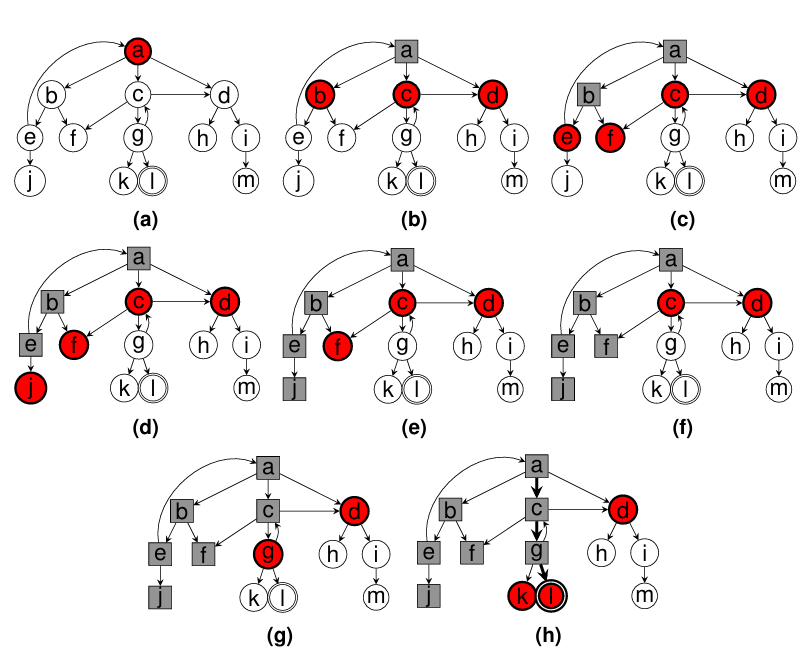
\includegraphics[width=0.8\textwidth]{./imgs/dfs.png}
	\caption{Depth First Search}
\end{figure}

\subsubsection{Pseudocode}
\begin{algorithm}[H]
	\caption{Depth First Search (\textit{start, goal})}\label{alg:dfs}
	\begin{algorithmic}[1]
	\State stack \(\gets\) [start]
	\While {stack is not empty}
		\State node \(\gets\) pop(stack)
		\If {node = goal}
			\State return path
		\EndIf
		\ForAll {neighbor in valid moves}
			\If {neighbor not visited}
				\State mark neighbor as visited
				\State push(stack, neighbor)
			\EndIf
		\EndFor
	\EndWhile
	\State return failure
	\end{algorithmic}
\end{algorithm}

\subsubsection{Implementation}

\subsubsection{Time and Space Complexity}